\documentclass[11pt,a4paper]{article}
\usepackage[margin=2.4cm]{geometry}
\usepackage{graphicx}
% Three search paths, so the document compiles from the repository (../figures/), from a
% flat Overleaf upload with the PNGs beside it (./), or with them in a subfolder.
\graphicspath{{../figures/}{figures/}{./}}
\usepackage{booktabs}
\usepackage{siunitx}
\usepackage{amsmath}
\usepackage[hidelinks]{hyperref}
\usepackage{caption}
\captionsetup{font=small,labelfont=bf}
\sisetup{detect-all,group-separator={,}}
\DeclareSIUnit{\mm}{mm}
\DeclareSIUnit{\km}{km}
\setlength{\parskip}{0.5em}
\setlength{\parindent}{0pt}

\title{Global hourly streamflow under daily-only supervision\\[0.3em]
  \large Phase I}
\author{Weikang Kong}
\date{2026-08-30}

\begin{document}
\maketitle
\begin{abstract}
\noindent
Hourly streamflow models are trained where hourly discharge is recorded, which is a small
and geographically narrow part of the world. Most gauges report once a day. This report
asks whether hourly skill survives at gauges that supply only daily totals. One fifth of a
network of nearly nine thousand gauges is held out, its hourly observations are hidden, and
only the 24-hour aggregate is used to supervise it. The hidden hourly series is read once,
to score. Daily aggregates recover most of the lost skill, and the recovery is a repair of
amplitude rather than of timing. The same result holds on 282 African catchments that
appear nowhere in training and genuinely lack hourly discharge. Part~I describes the
experiments. Part~II reports and analyses the results.
\end{abstract}
\tableofcontents
\clearpage
\part{Experiments}

\section{The problem, and how it is made testable}\label{sec:problem}
Hourly streamflow forecasting needs hourly discharge observations to train on. Those observations exist in a small part of the world. Most gauges that report at all report once a day. If a model trained on hourly data could keep its hourly skill at gauges that supply only daily totals, the usable domain would widen a long way.

The question is easy to state and hard to test, because a gauge either has hourly data or it does not. We make it testable by withholding. One fifth of the gauges are held out. Their hourly observations are hidden from training. Only the 24-hour aggregate is used to supervise them. The hidden hourly series is then read once, at the end, to score. Nothing in training ever sees it.

Three model states are compared throughout, and the whole report turns on them:
\begin{description}
  \item[M0] Zero-shot. The model is pretrained on the four fifths of gauges that keep their hourly data, then evaluated on the held-out fifth without having seen those gauges at all.
  \item[M1] The same model after fine-tuning on the held-out gauges' daily aggregates. This is the state the method is meant to deliver.
  \item[STEP 3] The four fifths re-scored after that fine-tuning, to measure what adapting to a daily-only domain costs where the model already worked.
\end{description}

The gap between M0 and M1 is the quantity of interest. It says how much of the hourly skill lost by hiding hourly data can be bought back with daily totals alone.

\section{Data}\label{sec:data}
The training network holds 8,979 gauges with hourly discharge, drawn from six national and regional archives: CAMELSH (5,115), BOMAustralia (1,804), LamaHCE (834), Japan (690), Germany (463), LamaHIce (73).

The geography of that network is a limitation worth stating at the outset. There is no gauge in Africa, none in South America, and none in mainland Asia. About four fifths of the gauges lie between \SI{30}{\degree} and \SI{60}{\degree} north. The word global in this report describes the model. It does not describe the gauge network. Section~\ref{sec:africa} exists because of this.

Forcing is hourly precipitation, temperature and potential evapotranspiration. Each sample gives the model the past 365 days at daily resolution and the past \SI{336}{\hour} at hourly resolution, and asks for the discharge at the target hour.

Two ways of building the daily input were available and both were run to completion. Run~A takes the prepared training batches as they are. Their daily branch is a 1000-step power-law subsample of the hourly record, dense near the target hour and sparse further back. Run~B rebuilds the windows from the raw hourly source and computes 365 genuine daily means.

The two are not interchangeable. Counting how the 1000 subsampled points fall across the 365 days shows why: 8 days carry all 24 hours, 176 days carry exactly one point, and 7 days carry none. A single instantaneous sample is a poor estimate of a daily mean for precipitation, where most hours are zero. The daily mean cannot be recovered from the subsample, so it has to be rebuilt from the source. Appendix~\ref{app:config} reports what this costs.

\section{Model and configuration}\label{sec:model}
The model is a shared multi-timescale LSTM with two branches. The daily branch reads 365 days and hands its hidden and cell state to the hourly branch at a transfer point set by the hourly look-back. The hourly branch reads forward from there and emits one value per hour. Training minimises a loss on the hourly targets where they are available, and on the 24-hour aggregate where they are not.

Two settings were changed together during development and both are reported. Configuration v1 used a \SI{72}{\hour} hourly look-back and the framework's default forget-gate initialisation. Configuration v2 uses \SI{336}{\hour} and an initial forget bias of 3. The forget gate matters more than its size suggests. At the default the effective forget gate sits at 0.500, which corresponds to a memory of roughly two steps. At bias 3 it sits at 0.953, roughly twenty-one steps. The published method this model follows specifies the latter. Its absence from v1 was an oversight. Configuration v3 repeats v2 with a longer epoch budget and is used only to check that v2 was not stopped early.

All configurations are reported together in Appendix~\ref{app:config}, rather than the best one being reported alone.

\section{Evaluation}\label{sec:evaluation}
A five-fold design gives every one of the 8,979 gauges exactly one turn as a held-out gauge. Target-domain scores therefore cover the whole network. No result depends on which fifth happened to be drawn.

Skill is reported as Kling-Gupta efficiency and Nash-Sutcliffe efficiency, both as medians across gauges. KGE is used for most of the analysis because it decomposes into three terms that answer separate questions:
\begin{equation}
  \mathrm{KGE} = 1 - \sqrt{(r-1)^2 + (\alpha-1)^2 + (\beta-1)^2},
  \qquad \alpha = \frac{\sigma_{\mathrm{sim}}}{\sigma_{\mathrm{obs}}},
  \qquad \beta = \frac{\mu_{\mathrm{sim}}}{\mu_{\mathrm{obs}}}.
\end{equation}
Here $r$ carries timing, $\alpha$ carries the amplitude of the variation, and $\beta$ carries the water balance. A drop in KGE alone says nothing about which of the three failed. The decomposition is what lets Section~\ref{sec:mechanism} say which one the method repairs.

The held-out fifth is drawn two ways. A random split leaves each held-out gauge a trainable neighbour \SI{10.4}{\km} away at the median. A blocked split, built from \num{120} k-means clusters on the sphere, pushes that to \SI{94.9}{\km}. Both were run with everything else identical. The difference between them measures how much of the zero-shot skill comes from genuine generalisation and how much comes from having a training gauge nearby. Fold-to-fold spread was recorded for both, and Section~\ref{sec:cost} reports why that turned out to matter as much as the level.

\section{External validation on Africa}\label{sec:africa-design}
Everything above simulates the premise. The hourly data exists and is deliberately hidden. Africa does not need the simulation, because the premise is the ordinary state of affairs there.

Of the African entries in the daily discharge database, \num{302} carry a time series at all. \num{294} of those are used here, and \num{282} pass a \num{100}-day minimum and are scored. That set is the test set of a published continent-holdout run, adopted unchanged so the numbers here sit directly against its baseline. No African catchment appears anywhere in pretraining. None has hourly discharge.

The pretrained models are driven over these catchments with hourly ERA5-Land forcing. Their last 24 hourly outputs are averaged to a daily value and compared with the observed daily discharge. Fine-tuning then uses African daily observations themselves, which makes the African M1 the direct analogue of the target-domain M1. ERA5-Land's own runoff is carried alongside as a physical baseline and re-scored on the identical basin-days, so all three numbers rest on the same observations.


\clearpage

\part{Results}

\section{Daily aggregates recover most of the lost hourly skill}\label{sec:main}
Under the primary configuration and a random split, median hourly KGE on the held-out gauges rises from \num{0.5190} at M0 to \num{0.6210} at M1. NSE rises from \num{0.5181} to \num{0.5896}. The paired median change in KGE is \num{+0.0623} over 8,979 gauges.

The median alone would be weak evidence. A few gauges with large gains can lift it while most gauges stay flat. They do not here. \SI{68}{\percent} of gauges improve. The effect is broad.

Under the blocked split the same fine-tuning lifts \num{0.4185} to \num{0.6165}. The zero-shot level is much lower there, and Section~\ref{sec:cost} explains why. The point for now is that both splits end at nearly the same place after fine-tuning, around \num{0.62}.

Figure~\ref{fig:map} puts every gauge on the map, before and after, together with the African basins that Section~\ref{sec:africa} discusses. Two things are visible at once. The gain is present across the whole network rather than in one region. And the network itself is temperate and northern. The empty continents in that figure are the reason the African test carries as much weight as it does.

\begin{figure}[htbp]
  \centering
  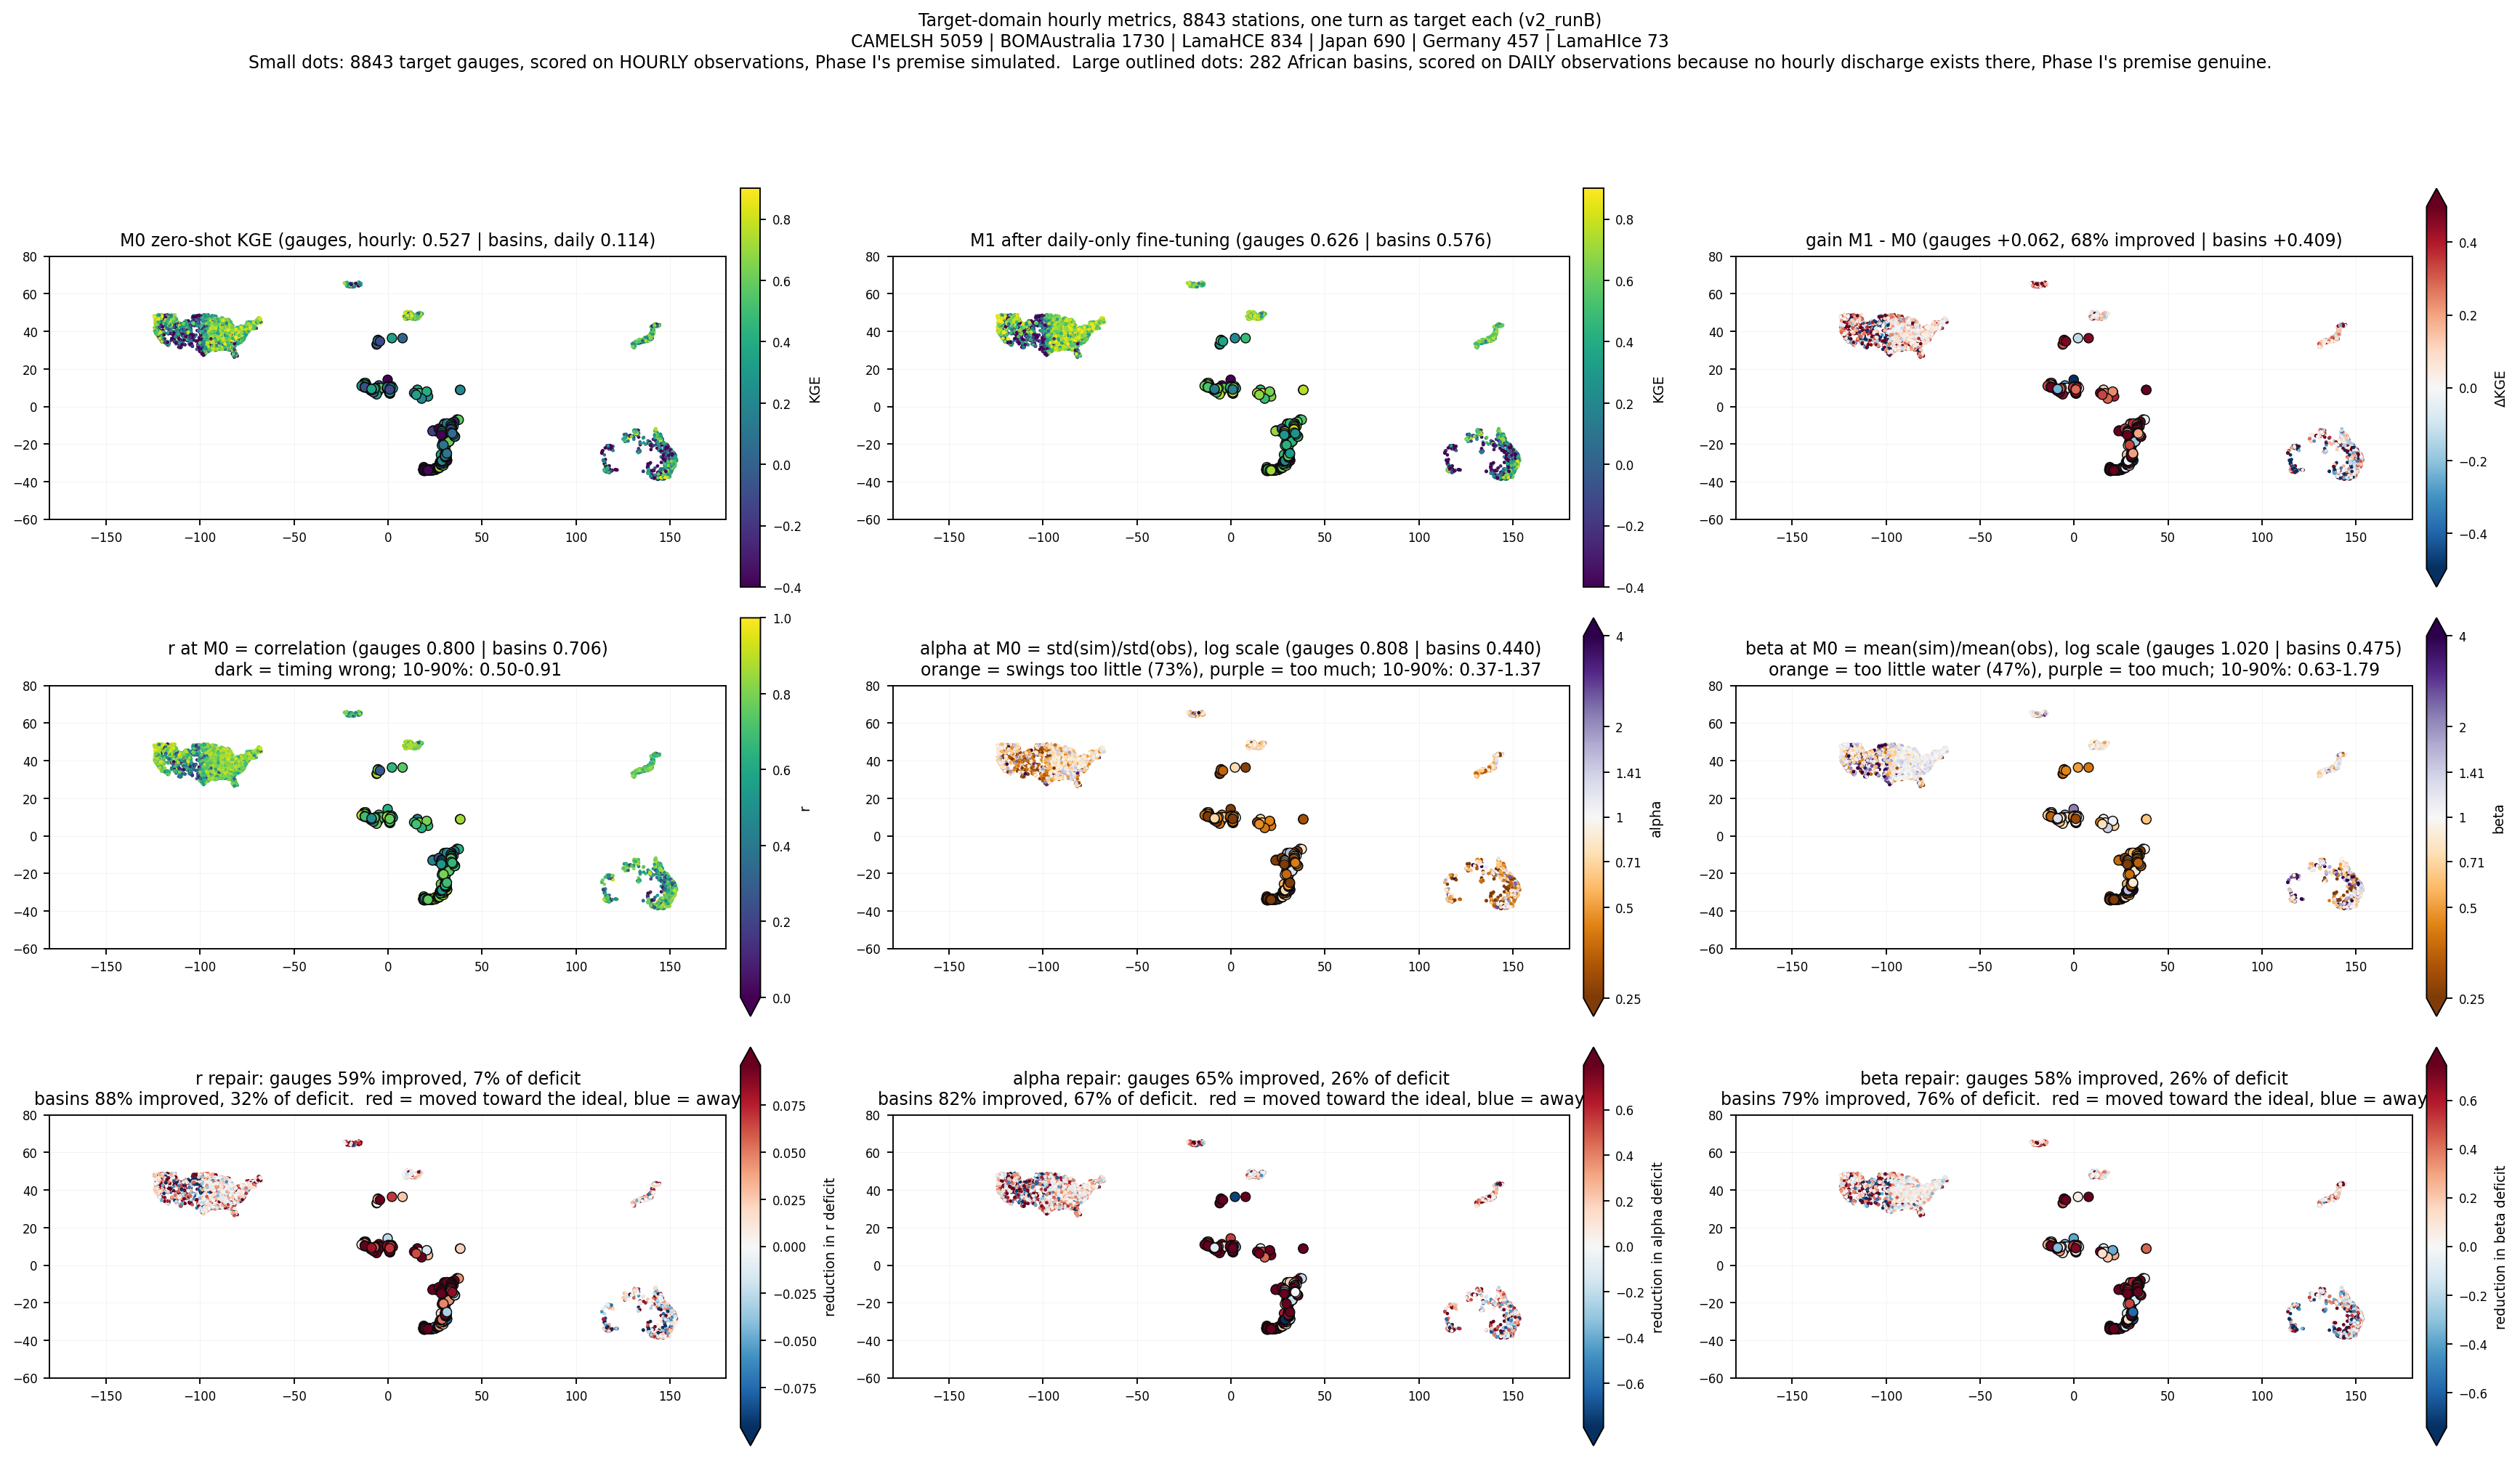
\includegraphics[width=\linewidth]{fig09_global_map.png}
  \caption{Columns are M0, M1 and their difference; rows are KGE and its three components, with the first two columns of a row sharing one scale. Small dots are the target gauges, scored against hourly observations, where Phase~I's premise is simulated; large outlined dots are the African basins, scored against daily observations, where it is genuine. The two are never pooled into one median because the observation each score rests on differs. $\alpha$ and $\beta$ use a log scale, so halving and doubling the observed value sit equally far from the white centre. Longitude is labelled on the bottom row and latitude on the left column only, since all twelve panels share one window. Panels: (a) KGE at M0, gauges 0.527, basins 0.114; (b) at M1, 0.626 and 0.576; (c) the difference, median +0.062 and +0.409.\ (d) $r$ at M0, gauges 0.800, basins 0.706; (e) at M1, 0.815 and 0.799; (f) the difference, median +0.005 and +0.080.\ (g) $\alpha$ at M0, gauges 0.808, basins 0.440; (h) at M1, 0.845 and 0.830; (i) the difference, median +0.037 and +0.333.\ (j) $\beta$ at M0, gauges 1.020, basins 0.475; (k) at M1, 0.995 and 0.953; (l) the difference, median -0.019 and +0.455. In the difference column the sign is the verdict for KGE and $r$, where larger is better, but not for $\alpha$ and $\beta$, whose ideal is 1.0: an increase helps a gauge below it and hurts one above it.}
  \label{fig:map}
\end{figure}

\section{The gain is a repair of amplitude}\label{sec:mechanism}
A 24-hour total carries how much water arrived on a day. It carries almost nothing about which hour it arrived in. If that is the whole of what the daily signal contributes, then fine-tuning on it should move the amplitude and water-balance terms of KGE and leave the correlation term nearly where it was. This is a prediction that can fail, and it is worth checking rather than assuming.

It holds. Correlation moves by \num{+0.0054}, from \num{0.797} to \num{0.812}. The amplitude ratio $\alpha$ moves by \num{+0.0370}. The water balance $\beta$ moves from \num{1.025} to \num{0.996}, that is, toward its ideal value of 1. Figure~\ref{fig:components} shows the three movements side by side under both splits, and Table~\ref{tab:deficits} gives the same comparison as distances from the ideal.

The diagnosis this gives is specific. A zero-shot model applied to an unseen catchment hedges toward the mean. Hedging minimises squared error under uncertainty, and it shows up as $\alpha$ below 1: the model swings less than the river does, and it flattens peaks. The daily total tells the model how much water a day actually carried, which is exactly the information needed to stop hedging. Timing was already close to right on this network, so there was little for the daily signal to add there even if it could.

\begin{figure}[htbp]
  \centering
  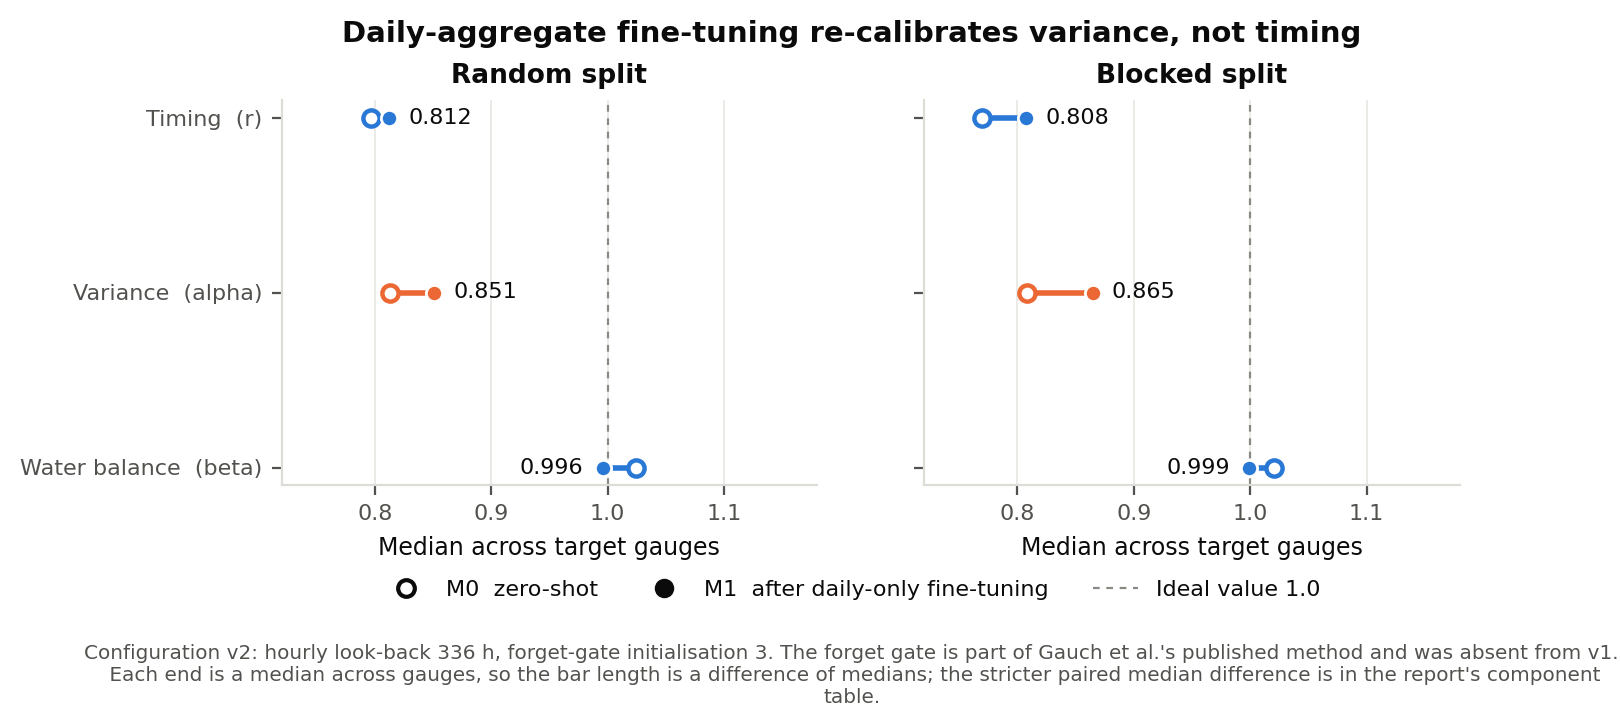
\includegraphics[width=\linewidth]{fig01_kge_components.png}
  \caption{Movement from M0 (open marker) to M1 (filled marker) in each KGE component, under both splits. Each end is a median across gauges. The correlation term barely moves. The amplitude term moves substantially. This is the finding that daily-aggregate supervision re-calibrates amplitude while leaving timing alone.}
  \label{fig:components}
\end{figure}

Appendix~\ref{app:mechanism} repeats this decomposition on the African catchments, whose zero-shot deficits are about four times larger. The same ordering holds there, which is the stronger version of the claim: it survives a domain that differs from this one by a wide margin.


\section{Three ways the gain could be false, and why it is not}\label{sec:falsify}
A gain measured this way could be an artefact in three separate ways. Each was given its own test before the result was believed.

\subsection{The model could be gaming the aggregate loss}
The aggregate term constrains only the mean of 24 hourly outputs. A model that emitted a constant value within each day would satisfy it perfectly and be useless at the hourly scale. This failure mode has to be excluded directly.

Stride-24 sampling makes each sample's last 24 outputs one calendar day, and consecutive days join into a continuous series. Within-day variability can then be measured against the observations.

The result is in Table~\ref{tab:degenerate}.

\begin{table}[htbp]
  \centering
  \caption{Within-day behaviour of the hourly output, as a ratio to the observed median across gauges. A flattened output would show ratios near zero in the first three rows.}
  \label{tab:degenerate}
  \begin{tabular}{lrrr}
    \toprule
    Quantity & Observed & M0 / obs & M1 / obs \\
    \midrule
    Flashiness & 0.0285 & 0.95 & 1.02 \\
    Within-day std & 0.0058 & 0.86 & 0.89 \\
    Within-day range & 0.0187 & 0.88 & 0.91 \\
    Q95 events / yr & 11.9395 & 0.99 & 1.02 \\
    Mean flow & 0.0483 & 1.05 & 1.03 \\
    \bottomrule
  \end{tabular}
\end{table}

The hourly output keeps its within-day variability, and it keeps close to the right amount of it. Configuration v1 failed this check in the opposite direction, with a zero-shot model \num{6.8} times too flashy and \num{3.1} times too variable within the day. The forget-gate initialisation removed that. Figure~\ref{fig:intraday} shows both configurations on one axis.

A sharper version of the question asks whether the hourly output responds to rainfall events or merely to the clock. Averaging every day by hour of day destroys event-driven structure, because storms keep no fixed hour. Whatever survives that average is tied to the clock. The observed average day has a peak-to-trough ratio of \num{1.044}, so the real river's average day is nearly flat. The model's is \num{1.098}, which is \num{1.05} times the observed amplitude. The model neither invents a daily cycle nor suppresses one.

\begin{figure}[htbp]
  \centering
  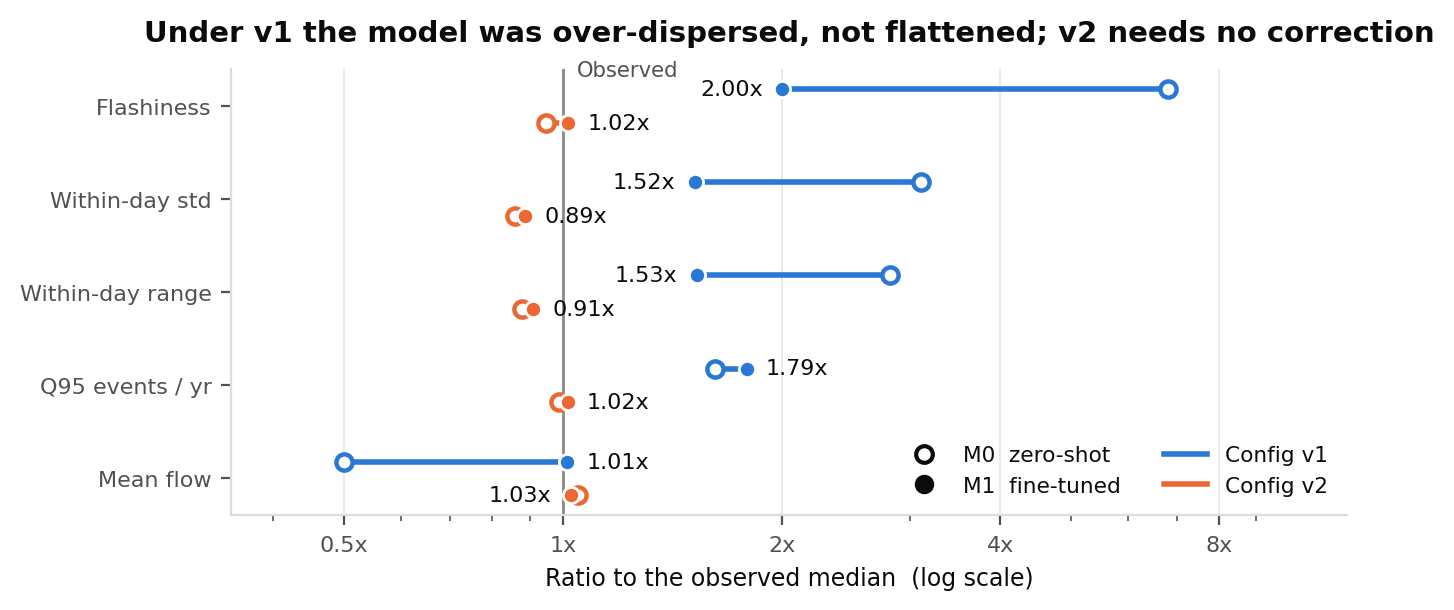
\includegraphics[width=\linewidth]{fig08_intraday_shape.png}
  \caption{Within-day behaviour as a ratio to the observed median, on a log scale, for both configurations. Configuration v1 was over-dispersed, which is a different failure from the flattening this check was built to catch. Configuration v2 is calibrated before fine-tuning and stays so after it.}
  \label{fig:intraday}
\end{figure}

\subsection{The improvement could be an artefact of the metric}
KGE and point-wise absolute error can move in opposite directions on the same gauge. They agree on about \SI{68}{\percent} of gauges here. Roughly a fifth improve on KGE while their point-wise error worsens, and about an eighth do the reverse.

This follows from the mechanism rather than undermining it. Restoring amplitude moves peaks. Moving a peak improves the shape metrics and can increase squared error at individual hours, particularly if the peak is slightly early or late. The practical consequence is that a per-gauge claim has to name its metric. Appendix~\ref{app:metrics} shows the joint distribution.

\subsection{The gain could be a training-budget artefact}
If the primary configuration had simply run out of epochs, its advantage over v1 would say more about the budget than the method. Configuration v3 answers this with a longer budget and higher patience. Early stopping ended every fold of v2 before the cap, and v3's extra epochs wander around the same plateau rather than climbing above it. Appendix~\ref{app:convergence} shows the curves.

The same run measures a cost the method imposes on itself. The checkpoint has to be chosen on a daily-aggregate criterion, because the hourly truth is meant to be hidden. Choosing on the hidden hourly truth instead would gain \num{0.0035} in median KGE. Fold-to-fold noise on the same quantity is \num{0.0078}. The cost of the constraint is smaller than the noise it would be measured against.

\section{What the method costs}\label{sec:cost}
Two costs are measurable and both are reported here rather than left to an appendix. A method whose price is unstated has not been evaluated.

\subsection{Adapting to the daily domain degrades the hourly domain}
Fine-tuning changes the weights, and those weights also serve the four fifths of gauges that kept their hourly data. Re-scoring that source domain after fine-tuning gives a clear answer. Median hourly KGE there falls from \num{0.6367} to \num{0.5452}, and median NSE from \num{0.6211} to \num{0.5298}. Paired gauge by gauge the median change is \num{-0.0539}, and it is negative in every fold. This is a property of the procedure rather than one fold's luck.

The mechanism of Section~\ref{sec:mechanism} explains it. Fine-tuning re-calibrates amplitude toward the daily-only domain. The source domain was already calibrated, so the movement that helps one hurts the other. Whether the trade is acceptable depends on deployment. Source gauges keep their hourly data and do not need the fine-tuned weights, so the two domains can be served by separate checkpoints. Mixing a fraction of source samples back into fine-tuning was tested and works as a dial between the two, damping the re-calibration and giving back part of the target-domain gain.

\subsection{A random split flatters the result twice}
Blocking the split costs the zero-shot model a paired median of \num{-0.0594} in KGE, which is \SI{11.0}{\percent} of its random-split level. \SI{63.7}{\percent} of gauges are worse, at Wilcoxon $p = \num{1.6e-168}$, and the drop is negative in all six archives. Some of what looks like zero-shot generalisation under a random split is proximity to a training gauge.

Daily-aggregate fine-tuning returns \SI{89.7}{\percent} of that loss. The residual at M1 is \num{-0.0061}. Figure~\ref{fig:split} breaks the recovery down by archive, and one archive stands out: Iceland, with \num{73} gauges, recovers only \SI{38}{\percent}. The sparsest network is where the method has the least to work with.

Table~\ref{tab:recovery} gives the same breakdown numerically.

\begin{table}[htbp]
  \centering
  \caption{The cost of spatial blocking per archive, and how much daily-aggregate fine-tuning returns.}
  \label{tab:recovery}
  \begin{tabular}{lrrrr}
    \toprule
    Archive & Gauges & Drop at M0 & Drop at M1 & Recovered \\
    \midrule
    Germany & 458 & -0.0730 & +0.0012 & 102\% \\
    LamaHCE & 834 & -0.1213 & -0.0017 & 99\% \\
    CAMELSH & 5,047 & -0.0501 & -0.0055 & 89\% \\
    BOMAustralia & 1,607 & -0.0644 & -0.0076 & 88\% \\
    Japan & 690 & -0.0719 & -0.0106 & 85\% \\
    LamaHIce & 73 & -0.1515 & -0.0942 & 38\% \\
    \bottomrule
  \end{tabular}
\end{table}

\begin{figure}[htbp]
  \centering
  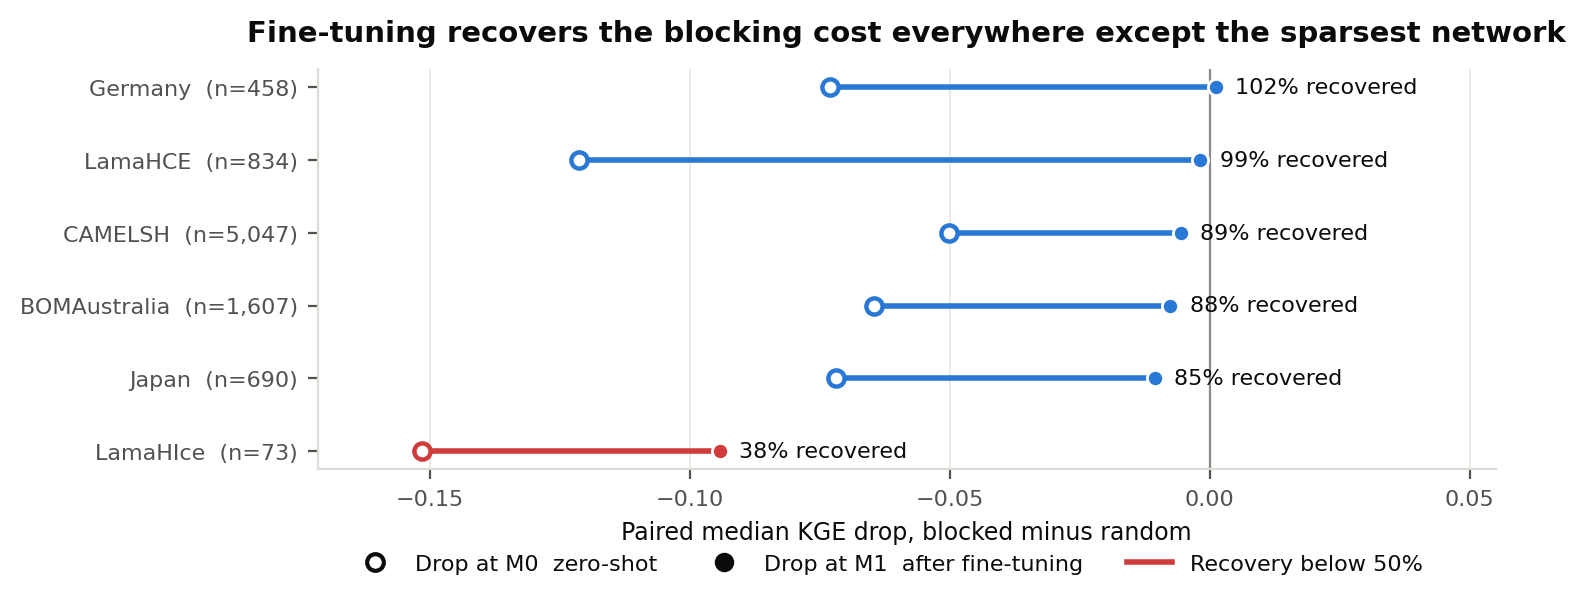
\includegraphics[width=\linewidth]{fig04_agency_recovery.png}
  \caption{Paired median KGE drop from blocking the split, per archive, at M0 (open marker) and after fine-tuning (filled marker). Every archive is negative at M0. Recovery exceeds \SI{85}{\percent} everywhere except the sparsest network.}
  \label{fig:split}
\end{figure}

A random split also overstates the precision of the result, which is easier to miss than the level. The fold-to-fold standard deviation of M1 is \num{0.0035} under the random split and \num{0.0411} under the blocked one, a factor of \num{11.8} at Levene $p = \num{0.034}$. Near-duplicate gauges sit on both sides of a random split, so its validation metric averages over fewer independent catchments than its gauge count suggests. The honest statement of the blocked result is about $0.62 \pm 0.04$. Quoting $0.628 \pm 0.004$ would be reporting the split's smoothness as if it were the model's stability.


\section{Africa, where the premise is real}\label{sec:africa}
Everything so far rests on hiding data that exists. That is a fair test of the method and a weak test of its reach, because the held-out gauges still sit inside a network the model was trained on. Africa provides the harder case. Its catchments appear nowhere in pretraining, and they genuinely lack hourly discharge.

Zero-shot performance there is poor, as expected for a continent absent from training: median KGE \num{0.1143}. Fine-tuning on African daily observations lifts it to \num{0.5761}. The paired median change is \num{+0.4094} with \SI{87.6}{\percent} of basins improving. The gain is roughly six times the one measured on the temperate network, which fits the mechanism: there was far more mis-calibration to repair.

Table~\ref{tab:threeway} places the three methods side by side.

\begin{table}[htbp]
  \centering
  \caption{All three scored on the identical \num{320540} basin-days over \num{282} basins. The ERA5-Land per-basin scores that already existed came from a different run over a different period, so they were recomputed here to make the comparison valid.}
  \label{tab:threeway}
  \begin{tabular}{lrr}
    \toprule
    Method & Median KGE & Median NSE \\
    \midrule
    ERA5-Land runoff & -0.3616 & -1.6762 \\
    M0, zero-shot & +0.1143 & +0.2028 \\
    M1, after African daily fine-tuning & +0.5761 & +0.5572 \\
    \bottomrule
  \end{tabular}
\end{table}

Two comparisons matter. Against the physical baseline, M1 beats ERA5-Land on \SI{93.6}{\percent} of basins, and even the zero-shot model beats it on \SI{76.2}{\percent}. Against the published continent-holdout baseline these basins were drawn from, which reaches a median KGE of \num{+0.2790}, M1 is higher by \num{+0.2971}.

Africa is also where one earlier claim needs qualifying. Across the temperate network the correlation term barely moved, and Section~\ref{sec:mechanism} attributed that to timing already being close to right. In Africa timing starts genuinely wrong, and there it does move. The refined statement is that a daily total fixes which day the water arrives, which repairs day-scale timing where it is broken. It still says nothing about which hour within that day.

\subsection{The hourly question that Africa cannot answer}
No African catchment has hourly discharge, so the hourly output there can be compared between series and never scored. Two things can still be established.

First, the hourly output carries real sub-daily structure. Across all \num{284} basins the within-day coefficient of variation is \num{0.1246} at M0 and \num{0.1053} at M1. Neither is near zero.

Second, daily-only supervision does flatten that structure to a measurable degree. The paired median change is \num{-0.0192}, about \SI{15}{\percent} of the zero-shot value, at Wilcoxon $p = \num{1.7e-04}$. Within-day variation rises in only \SI{40}{\percent} of basins. This cost had not previously been measured.

Whether that flattening removes real structure or spurious structure cannot be settled in Africa. On the temperate network, where hourly observations exist, the same step moved within-day standard deviation from \num{0.86} to \num{0.89} of observed, which is movement toward the observations.

ERA5-Land appears in the hourly panels as a contrast and not as a reference. It has no river routing, so its basin average is runoff leaving the soil column rather than water passing a gauge. On one catchment its instantaneous rate reaches \SI{199}{\mm\per\day} where the daily observation peaks near \num{20}, while its daily mean matches the observation closely. The volume is right and the distribution within the day is wrong. Its average day swings by a factor of \num{4.2} with a peak at 15:00 UTC, which is afternoon convective rainfall passed straight through. The model damps that clock-driven cycle \num{4.6}-fold across all \num{284} basins.

Figure~\ref{fig:africa-hourly} keeps the two resolutions apart for this reason. The left block can be scored. The right block cannot, and saying so on the figure is the honest way to present it.

\begin{figure}[htbp]
  \centering
  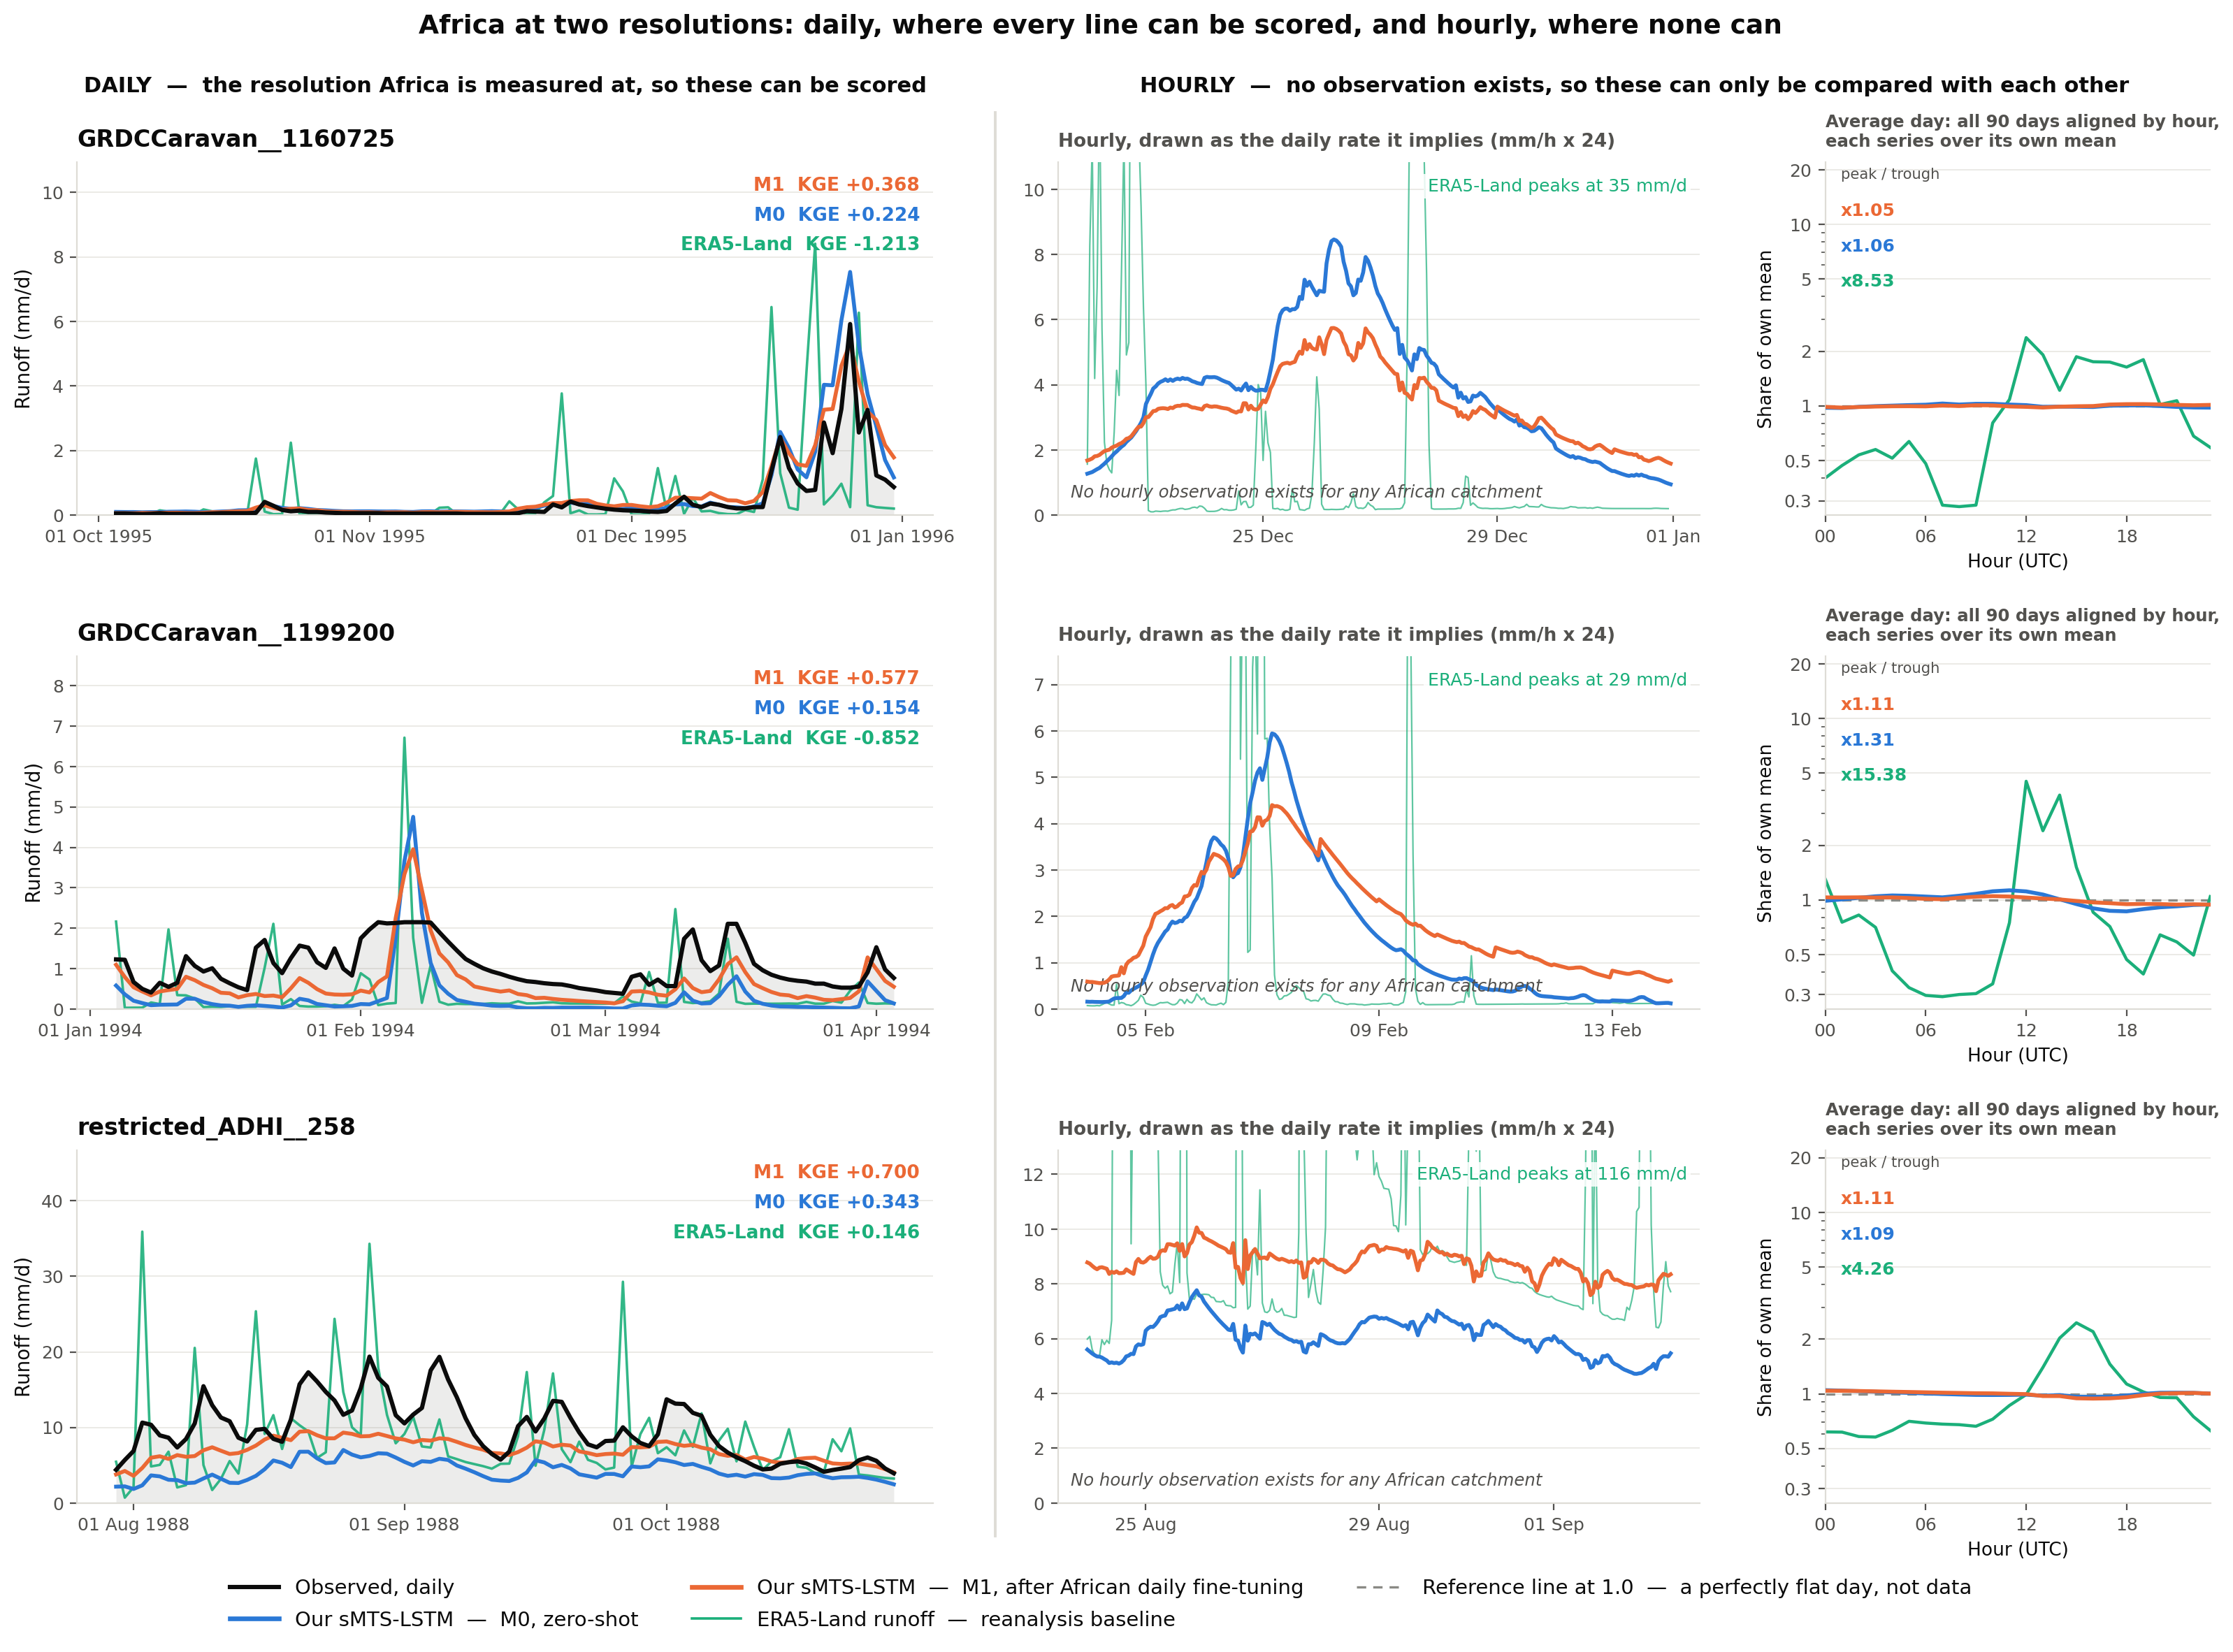
\includegraphics[width=0.98\linewidth]{fig10_africa_hourly.png}
  \caption{Africa at two resolutions, kept apart because only one of them can be scored. Left: daily, where the observation exists and every line carries a score. Right: hourly, where no observation exists anywhere on the continent, so the series can only be compared with each other. The rightmost panel aligns every day of the window by hour of day and divides each series by its own mean. A flat line there means no dependence on the clock.}
  \label{fig:africa-hourly}
\end{figure}

\section{What Phase I establishes}\label{sec:summary}
The result is that daily aggregates recover most of the hourly skill lost by hiding hourly observations, on a temperate network of nearly nine thousand gauges and on two hundred and eighty-two African catchments that were never in training. The repair is one of amplitude, and that holds on two domains whose deficits differ by about a factor of four. It survives the three checks of Section~\ref{sec:falsify}.

Four limits belong beside that result.
\begin{enumerate}
  \item Under-dispersion is reduced and not removed. \SI{74}{\percent} of gauges remain under-dispersed after fine-tuning, so this does not yet deliver a model to trust on peak magnitude.
  \item The adaptation degrades the source domain, by a paired median of \num{0.054} in KGE, in every fold.
  \item A random split overstates both the level and the precision of the result. Blocked-split numbers with their honest spread are the ones to quote.
  \item The training network is temperate and northern. The African test is the only genuinely external evidence here, and it rests on the \num{302} records that are all the daily database holds for the continent.
\end{enumerate}

\clearpage

\appendix
\part{Appendix}

\section{Configuration and data path}\label{app:config}
Run~A takes the prepared batches as they are, and it moves backwards under both configurations: median KGE falls from \num{0.427} to \num{0.397} under v1 and from \num{0.424} to \num{0.397} under v2. Every run~B variant gains. The daily branch in run~A is a power-law subsample rather than a series of daily means, so the daily-aggregate signal has no matching structure to attach to. No hyperparameter recovers this, which is why the whole report uses run~B.

Within run~B, v1 to v2 lifts the blocked split from \num{0.475} to \num{0.621}, and v3's longer budget changes almost nothing.

That step changes two settings at once, so it cannot say which one acts. Two pairs in the hyperparameter search differ in exactly one key, verified key by key rather than assumed from their names, and they separate the two effects. On M1, forget gate 0 -> 3 contributes \num{+0.0094} and hourly look-back 72 -> 336 contributes \num{+0.0467}. The look-back is the larger by roughly fivefold.

Each of those configurations ran \num{1} fold, so both are point estimates with no between-fold spread, judged against a fold-level noise floor of \num{0.0078} measured elsewhere in this work. The forget-gate effect clears that floor only narrowly. A five-fold ablation is required to settle the split and is in progress.

The forget gate is retained regardless of how the credit divides. It is part of the published method this model follows, and its absence from v1 was an oversight.

Figure~\ref{fig:config} shows all of them together.

\begin{figure}[htbp]
  \centering
  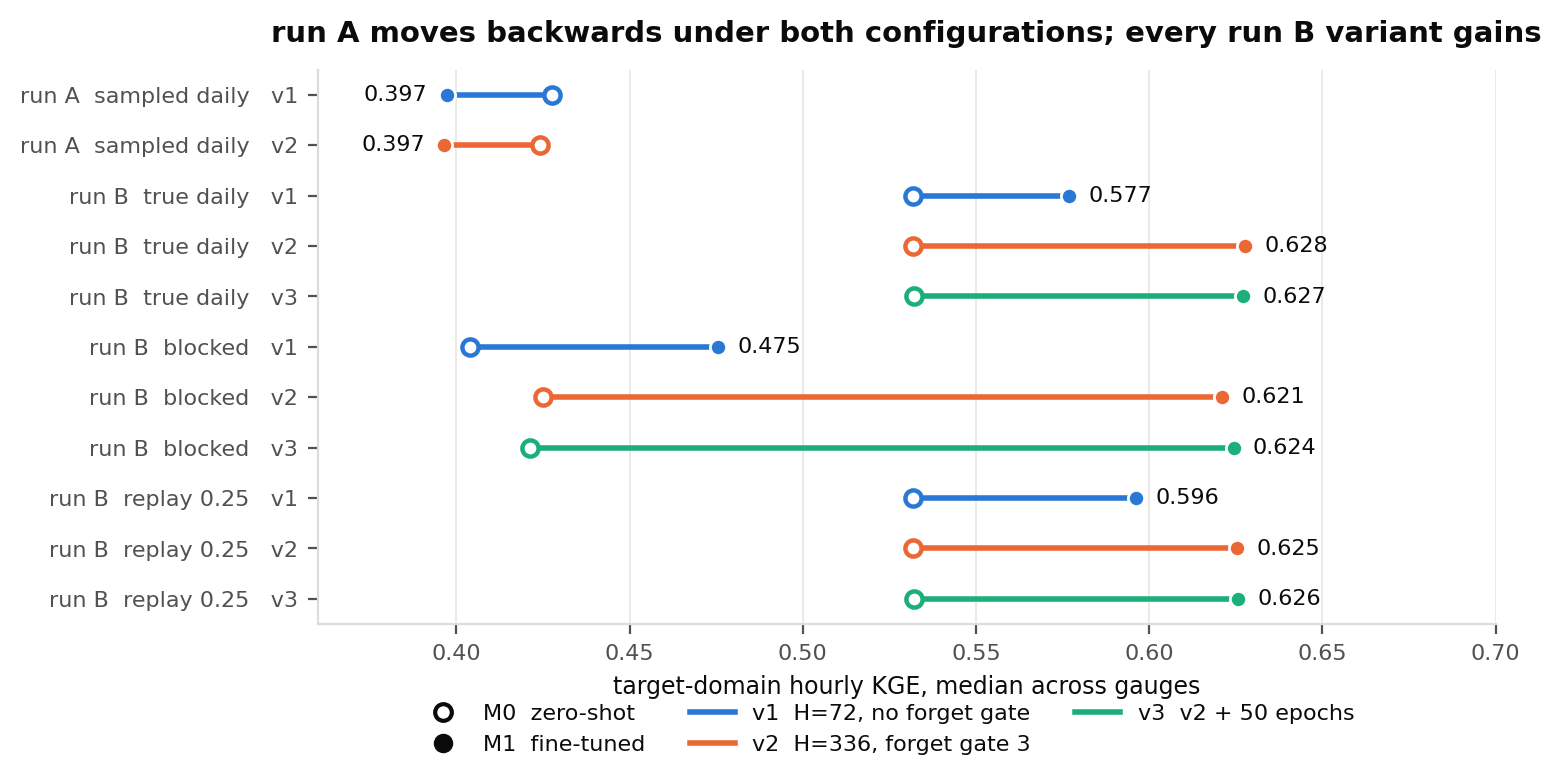
\includegraphics[width=\linewidth]{fig03_configurations.png}
  \caption{Every configuration as a movement from M0 (open marker) to M1 (filled marker) in median target-domain hourly KGE. Run~A is the only data path that moves backwards.}
  \label{fig:config}
\end{figure}

\section{Where the gain lands}\label{app:strata}
Small catchments gain most, at Spearman $\rho = \num{-0.172}$ against area over \num{8843} gauges. The gain falls from \num{0.112} in the smallest quintile to \num{0.022} in the largest. This fits the mechanism, because a small fast-responding catchment is where a zero-shot model is least calibrated.

Isolation does the opposite of what a proximity-driven result would do. Under the blocked split the gain rises with distance to the nearest trainable gauge, at $\rho = \num{+0.047}$. Being far from training data does not reduce what a daily total is worth.

Figure~\ref{fig:strata} shows both relationships.

\begin{figure}[htbp]
  \centering
  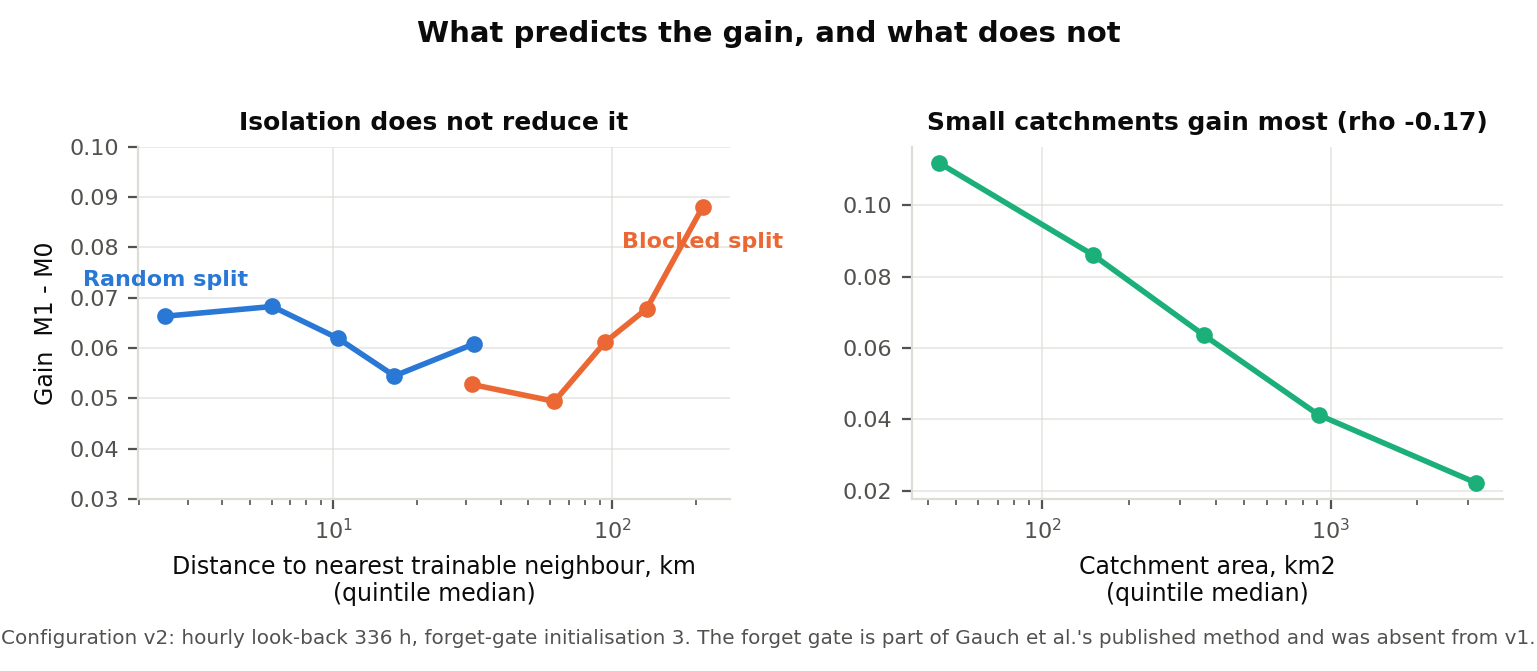
\includegraphics[width=\linewidth]{fig02_gain_drivers.png}
  \caption{Median gain by quintile, against distance to the nearest trainable gauge (left, one line per split) and against catchment area (right).}
  \label{fig:strata}
\end{figure}

\section{The mechanism across two domains}\label{app:mechanism}
Table~\ref{tab:deficits} states it numerically and Figure~\ref{fig:mechanism} draws it.

\begin{table}[htbp]
  \centering
  \caption{Distance from the ideal before and after fine-tuning. Deficit is $1-r$ for the correlation and $|\log_2 x|$ for the two ratios, because $0.5$ and $2.0$ are equally wrong for a ratio and their arithmetic mean is not 1. Only the fraction removed is comparable across components.}
  \label{tab:deficits}
  \begin{tabular}{lrrrr}
    \toprule
    Domain & Component & Deficit at M0 & Deficit at M1 & Removed \\
    \midrule
    target domain & $r$ (timing) & 0.203 & 0.188 & 7\% \\
    target domain & $\alpha$ (amplitude) & 0.464 & 0.342 & 26\% \\
    target domain & $\beta$ (water balance) & 0.280 & 0.211 & 25\% \\
    Africa & $r$ (timing) & 0.294 & 0.201 & 32\% \\
    Africa & $\alpha$ (amplitude) & 1.209 & 0.394 & 67\% \\
    Africa & $\beta$ (water balance) & 1.169 & 0.274 & 77\% \\
    \bottomrule
  \end{tabular}
\end{table}

The ordering is the same on both domains. target domain removes \SI{25}{\percent} of the amplitude and water-balance deficit against \SI{7}{\percent} of the timing deficit; Africa removes \SI{72}{\percent} of the amplitude and water-balance deficit against \SI{32}{\percent} of the timing deficit.

\begin{figure}[htbp]
  \centering
  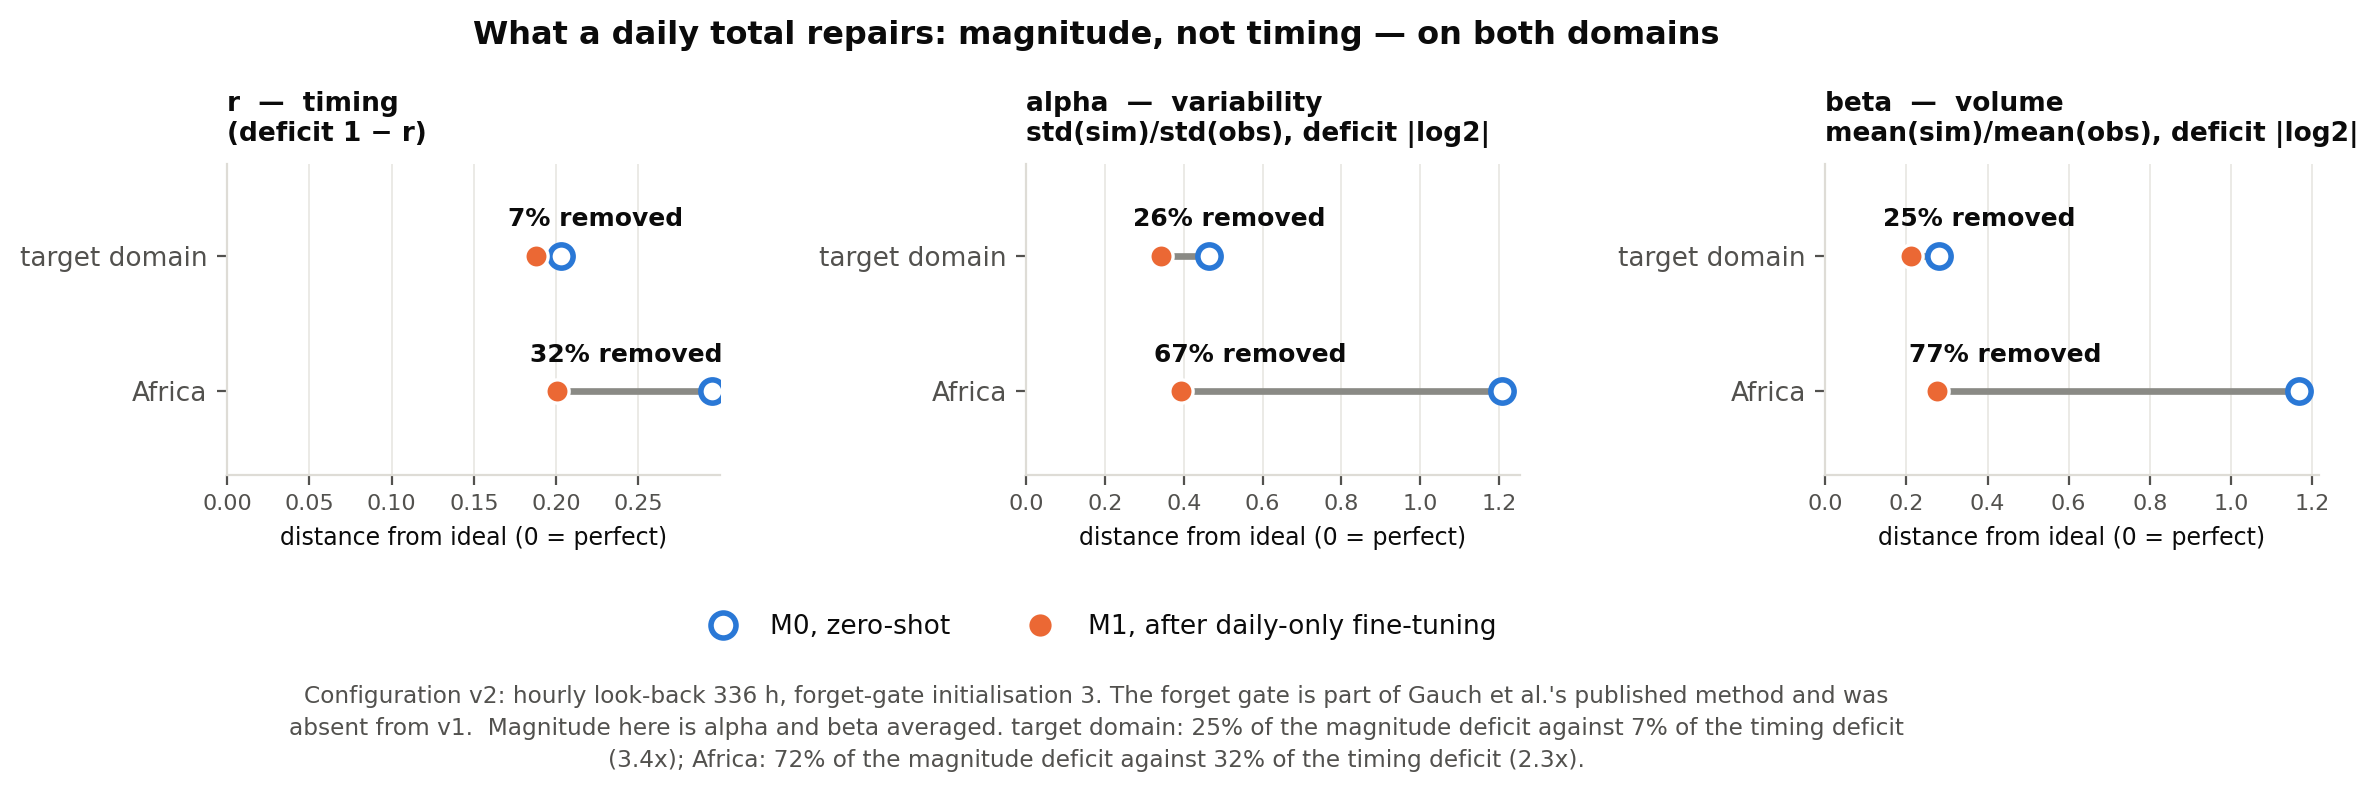
\includegraphics[width=0.95\linewidth]{fig11_component_deficits.png}
  \caption{One axis per component, because $1-r$ and $|\log_2 x|$ are in different units. The fraction removed, printed on each pair, is the comparable quantity.}
  \label{fig:mechanism}
\end{figure}

\section{Where the two metrics disagree}\label{app:metrics}
Figure~\ref{fig:metrics} shows the joint distribution behind the disagreement reported in Section~\ref{sec:falsify}.

\begin{figure}[htbp]
  \centering
  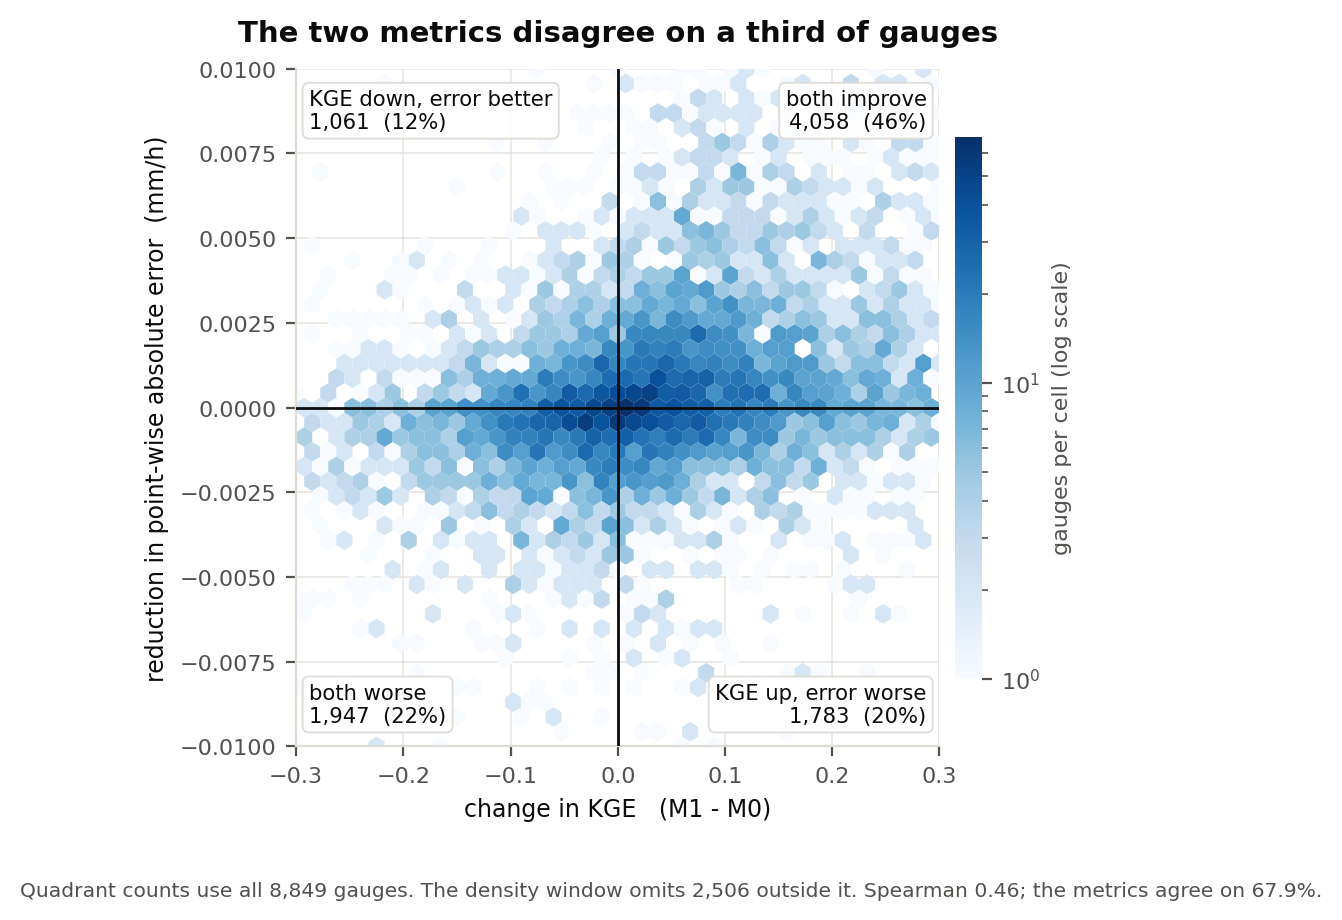
\includegraphics[width=0.72\linewidth]{fig05_metric_disagreement.png}
  \caption{Change in KGE against reduction in point-wise absolute error, one hexagon per group of gauges. Quadrant counts use every gauge. The density window omits those outside it, which the caption states rather than folding them into the corner bins.}
  \label{fig:metrics}
\end{figure}

\section{Training length}\label{app:convergence}
Figure~\ref{fig:convergence} shows the validation curves.

\begin{figure}[htbp]
  \centering
  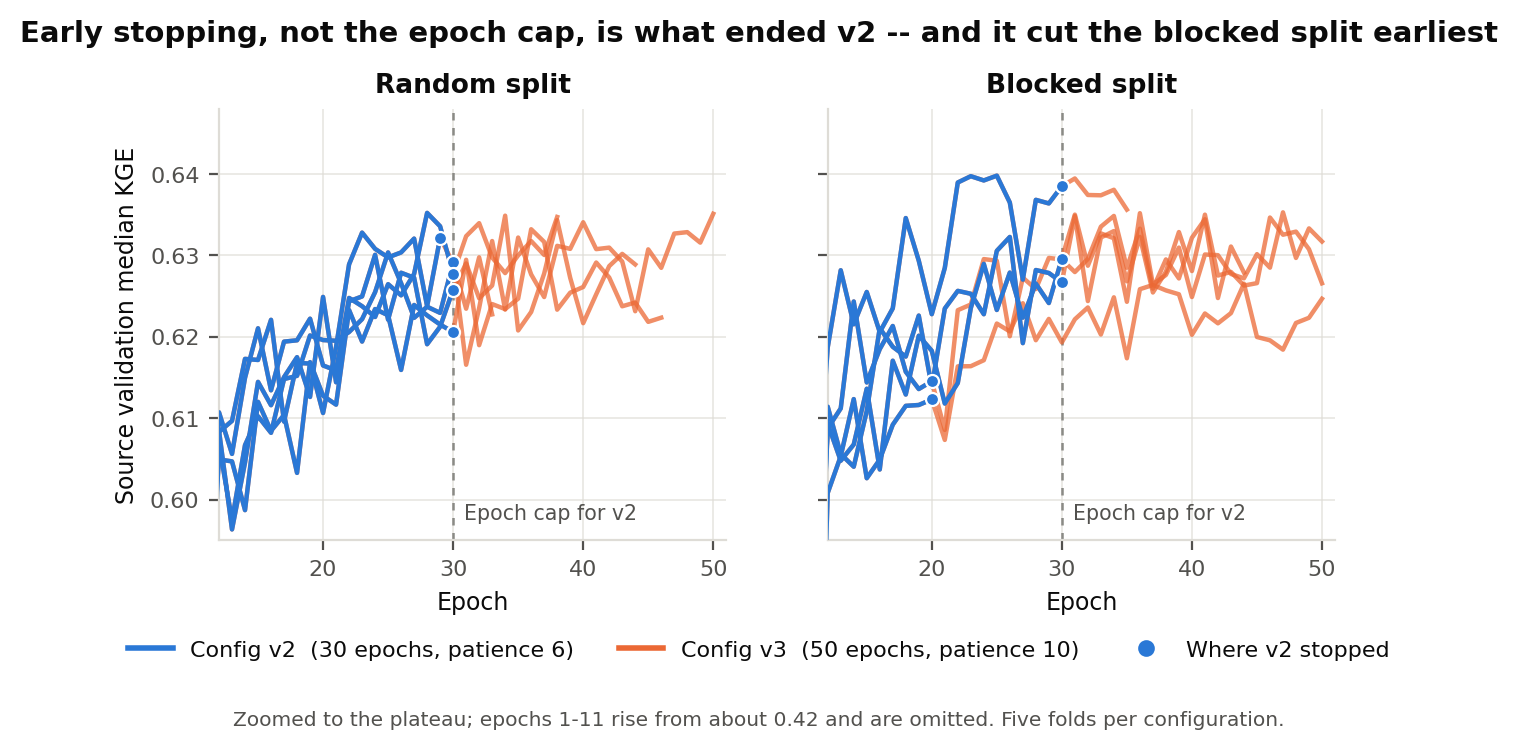
\includegraphics[width=\linewidth]{fig06_convergence.png}
  \caption{Source-domain validation KGE per epoch, five folds per configuration, zoomed to the plateau. The epochs at which v2 stopped are marked, and none reaches the cap.}
  \label{fig:convergence}
\end{figure}

\section{African hydrographs at daily resolution}\label{app:africa-daily}
Figure~\ref{fig:africa-daily} shows three of the catchments behind the daily numbers in Section~\ref{sec:africa}.

\begin{figure}[htbp]
  \centering
  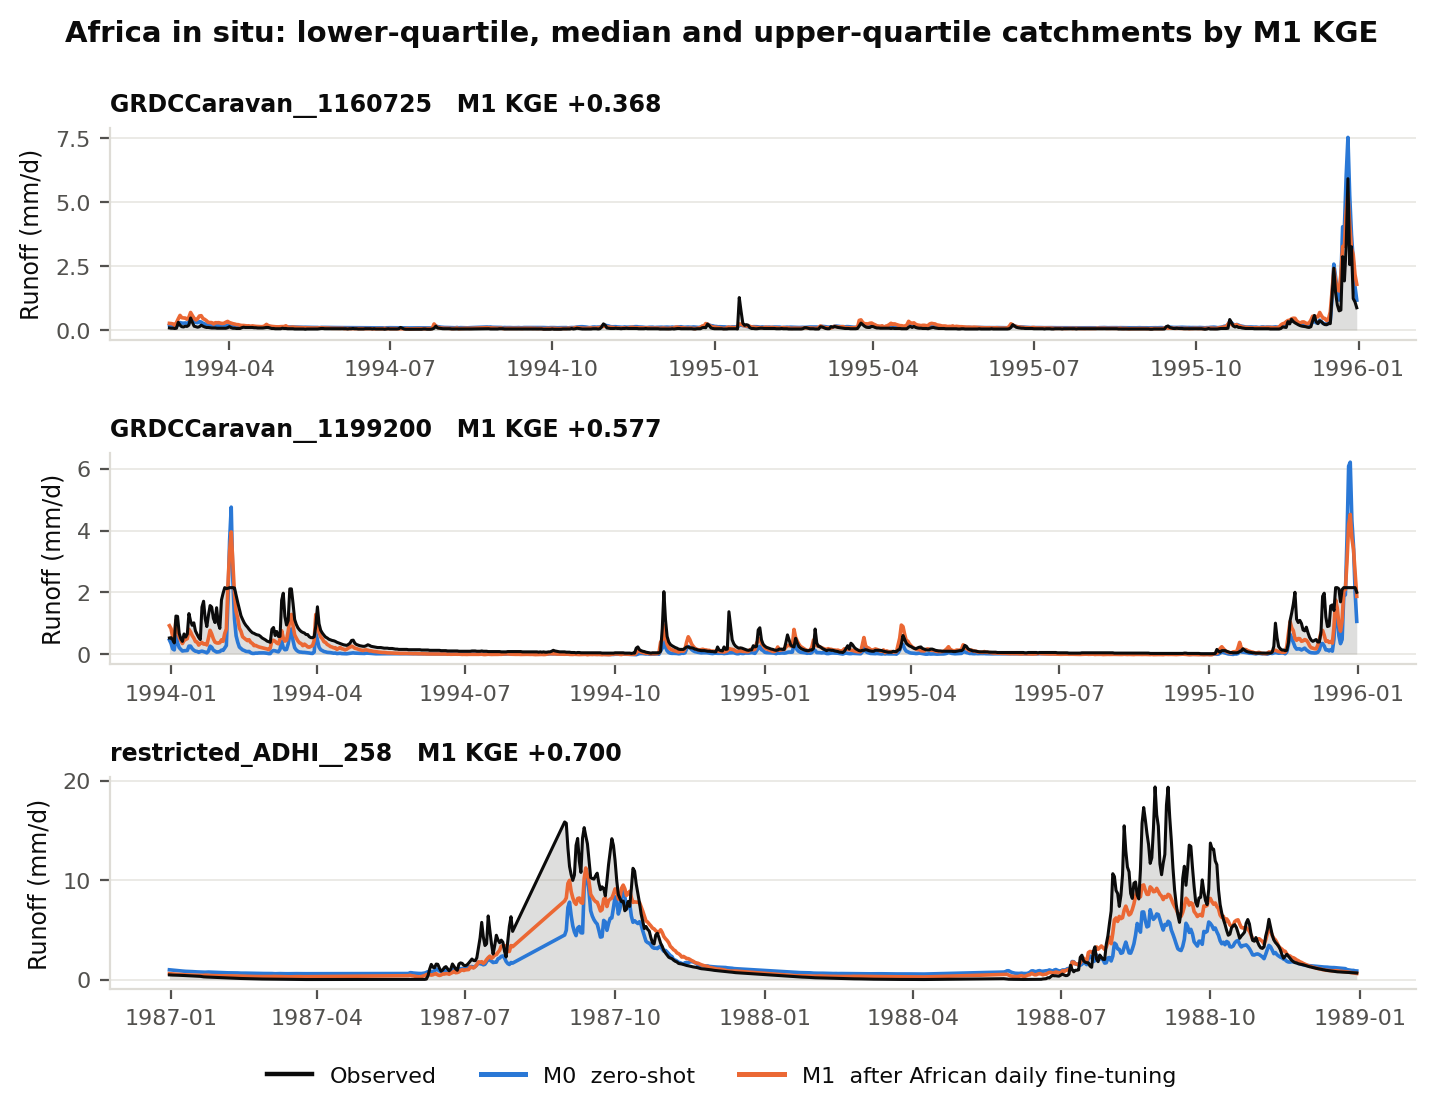
\includegraphics[width=0.86\linewidth]{fig07_africa_hydrographs.png}
  \caption{Three catchments spanning the outcome rather than three good ones: the lower-quartile, median and upper-quartile catchment by M1 KGE. The zero-shot model under-predicts every peak, and fine-tuning lifts them toward the observed hydrograph.}
  \label{fig:africa-daily}
\end{figure}


\end{document}
